
\documentclass[11pt]{beamer}

% contains the complete preamble
\usepackage{present}
\usepackage{custom_underline}
         		               		
\title{}
\author[Felix Z.~Hoffmann]{Felix Z.~Hoffmann}
\institute{}
\date{\today}     


\begin{document}


%% \begin{frame}{Bordeaux18 talk}

  

  
  
\end{frame}


%% % pre-Intro: About me - what qualifies me to tell you
%% % anything about reproducibility/open science. Whom am
%% % I to talk?
%% 
\begin{frame}{Who am I?}
  % 
  \begin{columns}
    %
    \begin{column}{.625\textwidth}
      \minipage[c][0.65\textheight][s]{\columnwidth}

      PhD student with Prof.~Jochen Triesch
      \vspace{0.15cm}
      
\begin{tabular}{|p{0.9\textwidth}}
      \textit{Computational models of structural plasticity}
\end{tabular}	     
  

      \vfill

      Google Summer of Code 2014
      \vspace{0.15cm}

      \begin{tabular}{|p{0.9\textwidth}}
        \textit{Data-centric views in Sumatra}
      \end{tabular}	     

      \vfill

      Wikimedia Open Science Fellow 2017/2018
      \vspace{0.15cm}

      \begin{tabular}{|p{0.9\textwidth}}
        \textit{Open computational research study}
      \end{tabular}	     

      
      
      \endminipage      
    \end{column}
    %
    \begin{column}{.249\textwidth}
      \minipage[c][0.7\textheight][s]{\columnwidth}

      \begin{figure}
        \centering
        \includegraphics[width=\textwidth]{%
          logo_fias+mpi.png} %
      \end{figure}
      
      \begin{figure}
        \centering
        \includegraphics[width=\textwidth]{%
          logo_gsoc14.jpg} %
      \end{figure}

      \begin{figure}
        \centering
        \includegraphics[width=\textwidth]{%
          logo_wosf.png} %
      \end{figure}
      \endminipage      

      
      
    \end{column}
  \end{columns}
  %  
\end{frame}




%% % Intro: Why we (might) need to do things differently
%% % from our supervisors/how it's been done until now
%% % reproducibility crisis everywhere !!
%% \begin{frame}{The reproducibility crisis}

  \begin{figure}
    \centering
    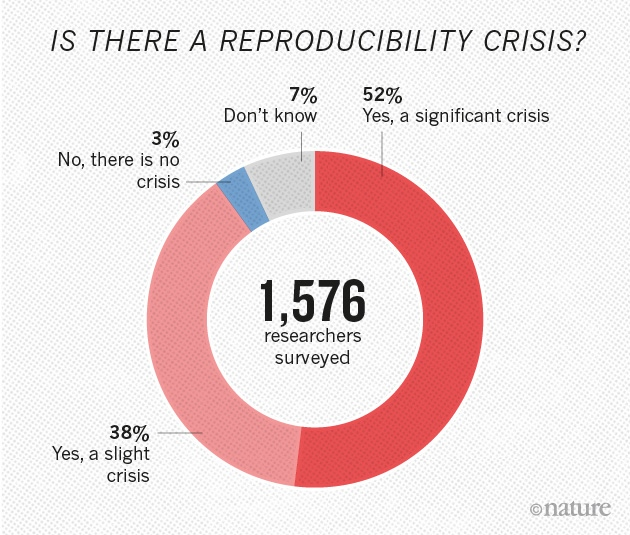
\includegraphics[width=0.85\textwidth]{%
    img/reproducibility_crisis_q.jpeg} %
  \end{figure}
  

  
  
\end{frame}



%% % So let's talk about code. Probably all of us are working
%% % with code, even if it's just a simple MATLAB script.
%% %
%% % What does reproducibility for these computational parts
%% % look like?
%% % 
%% % Naively, reproducibility shouldn't be a problem at all for code,
%% % right?
%% %
%% % 1. everyone has a computer (as opposed to a lab setup) and
%% %    running code is inexpensive and unproblematic compared
%% %    to replicating experiment
%% % 2. can share all the code (~5MB) opposed to sharing a full
%% %    lab (impossible)
%% % 
%% % So where's reproducibility in the computational sciences at?
%% % Well, it's not looking great.
%% %
%% % Many of you probably know from personal experience that this
%% % that this naive thinking does not apply, but let's look at
%% % how bad it really is:
%% %
%% % Problems:
%% % ---> study from Stodden and Collberg
%% 
\begin{frame}{Computational reproducibility should be easy...}

  % 
  \begin{columns}
    %
    \begin{column}{.5\textwidth}
      \begin{figure}
        \centering
        \includegraphics[width=0.85\textwidth]{%
          monkey.png}  %
      \end{figure}
      
    \end{column}
    %
    \begin{column}{.5\textwidth}

      \begin{figure}
        \centering
        \includegraphics[width=0.85\textwidth]{%
          computer.png}  %
      \end{figure}
      
    \end{column}
  \end{columns}

  \begin{columns}
    %
    \begin{column}{.5\textwidth}
      \begin{center}
        Hard
      \end{center}
      
    \end{column}
    %
    \begin{column}{.5\textwidth}
      \begin{center}
        Easy?
      \end{center}
      
    \end{column}
  \end{columns}
  
\end{frame}


\begin{frame}{Computational reproducibility should be easy...}

  \vspace{0.7cm}
  
  \begin{itemize}[leftmargin=1.2cm, rightmargin=1cm]

    \itemsep10pt

  \item[1.] cheap and universal access to computers (as opposed to a lab)
  \item[2.] running code is inexpensive and unproblematic (compared to replicating an experiment)
  \item[3.] can easily share code \& data that allow direction reproduction
    % 1. everyone has a computer (as opposed to a lab setup) and
    %    running code is inexpensive and unproblematic compared
    %    to replicating experiment
    % 2. can share all the code (~5MB) opposed to sharing a full
    %    lab (impossible)
    
    
  \end{itemize}


  

  % 
  \begin{columns}
    %
    \begin{column}{.625\textwidth}
      \minipage[c][0.45\textheight][s]{\columnwidth}

      \vspace{1.2cm}
      \begin{center}
        \textit{Is a there a reproducibility crisis\\ in computational research?}
      \end{center}        
      
      \endminipage      
    \end{column}
    %
    \begin{column}{.375\textwidth}
      \onslide<1->
      \vspace{-1cm}
      \begin{figure}
        \centering
        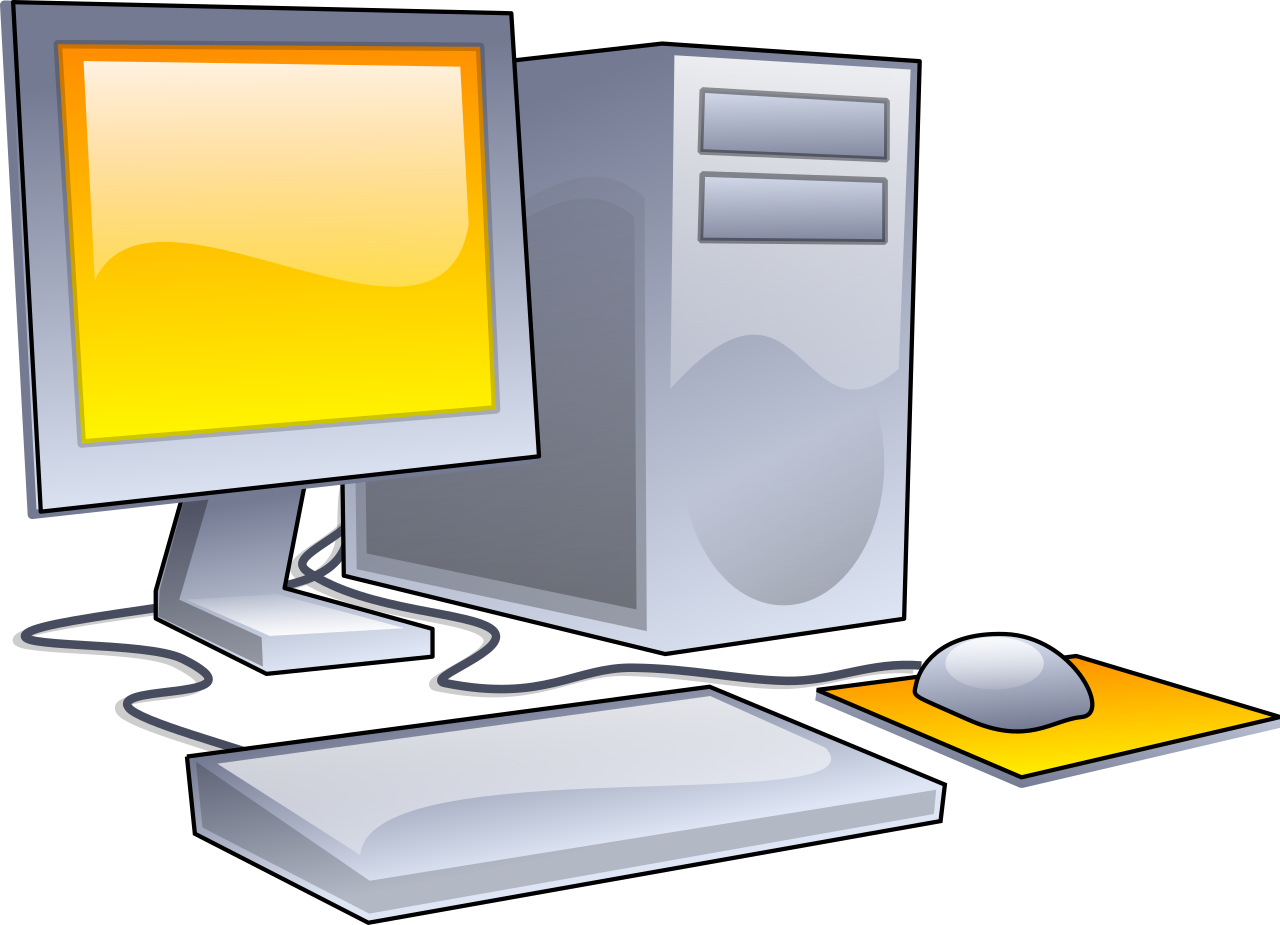
\includegraphics[width=\textwidth]{%
          img/computer.png} %
      \end{figure}
      
      
      
    \end{column}
  \end{columns}
  


  \pnote{
    
    But as many of you have probably experienced,\\
    code is often not shared.\\

    But surely, journals implementing policies \\
    should help?

    Well, let's take a look:
    
  }


  
  
\end{frame}



\begin{frame}{Sharing of code \& data mandatory in many journals}

  
  \begin{figure}
    \centering
    \includegraphics<1>[width=0.95\textwidth]{%
      img/science_policy.png} %
    \includegraphics<2>[width=0.95\textwidth]{%
      img/science_policy_t1.png} %
    \includegraphics<3>[width=0.95\textwidth]{%
      img/science_policy_t2.png} %
  \end{figure}

  \vspace{0.4cm}
  
  \begin{flushright}
    \small Policy of \textit{Science} since February 11, 2011
  \end{flushright}

  \pnote{
    
    Now that we established computational reproducibility\\
    should be simple and journals are demanding\\
    sharing anyway, we're good, right?

    How effect is such an policy?
    
  }
  
\end{frame}

\begin{frame}{}
  
  \begin{figure}
    \centering
    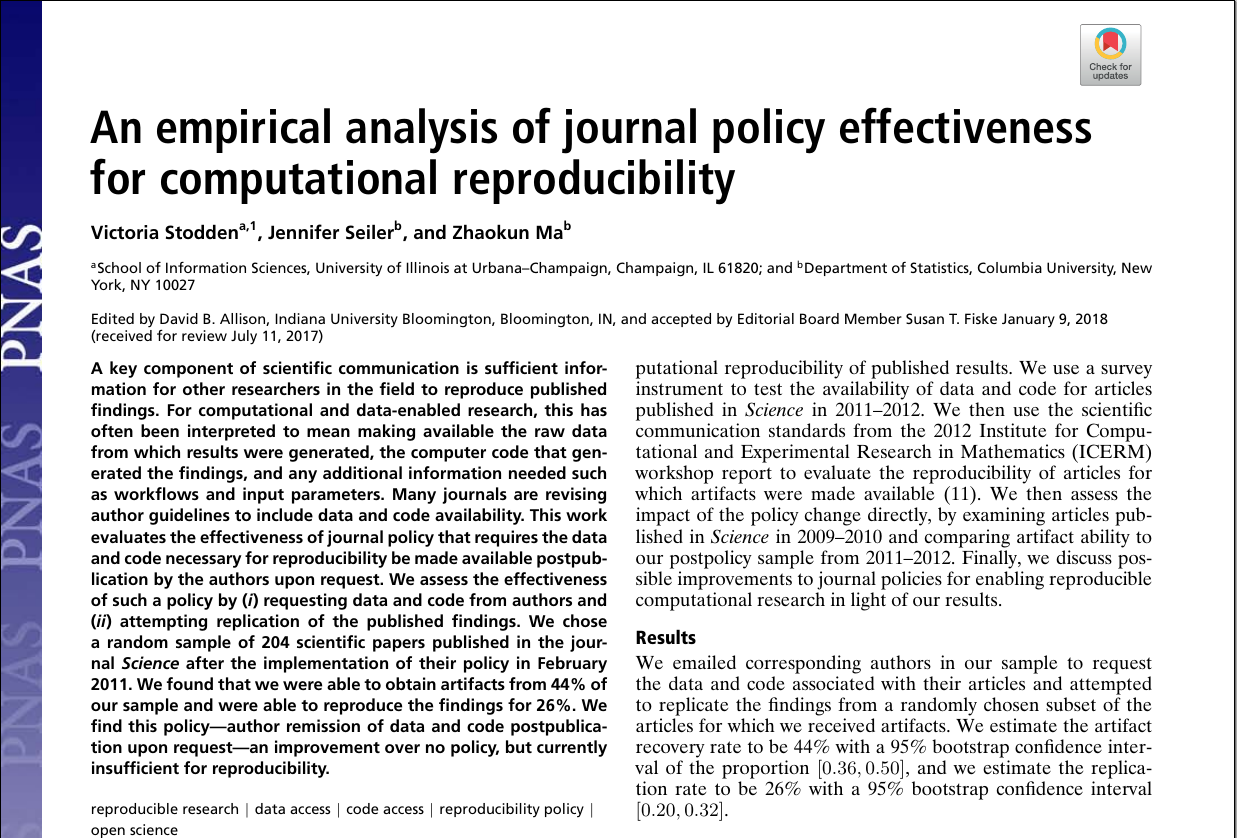
\includegraphics[width=0.875\textwidth]{%
      img/stodden2018_cover3.png} %
  \end{figure}
  
  \vspace{0.015cm}

  \begin{center}
    Out of 206 computational studies in \textit{Science} since 2011, \\
    26 provided code \& data directly  
  \end{center}
  

  \source{\cite{Stodden2018}}

  \pnote{
    
    To the remaining 180 studies \\
    the authors sent Emails asking \\
    for the code for the studies
    
  }

  
\end{frame}


\begin{frame}{A few responses...}
  
  \begin{figure}
    \centering
    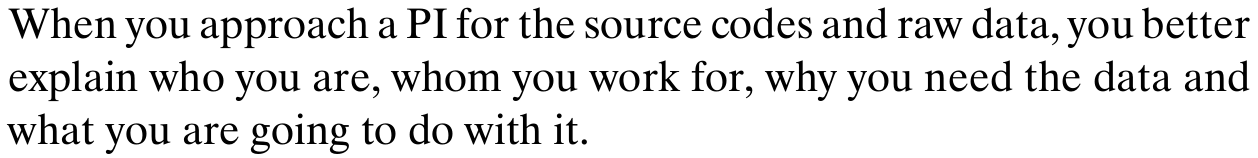
\includegraphics[width=0.95\textwidth]{%
      img/stodden2018_re1.png} %
  \end{figure}

  \begin{figure}
    \centering
    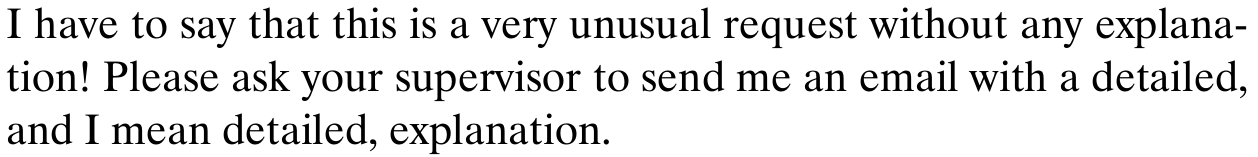
\includegraphics[width=0.95\textwidth]{%
      img/stodden2018_re2.png} %
  \end{figure}

  \begin{figure}
    \centering
    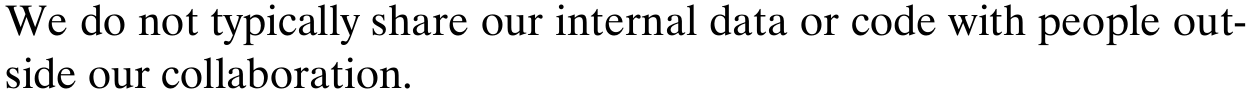
\includegraphics[width=0.95\textwidth]{%
      img/stodden2018_re3.png} %
  \end{figure}

  \source{\cite{Stodden2018}}
  
\end{frame}



\begin{frame}{\large   Of $N=206$ articles published in \textit{Science} since 2011...}


  \begin{figure}
    \centering
    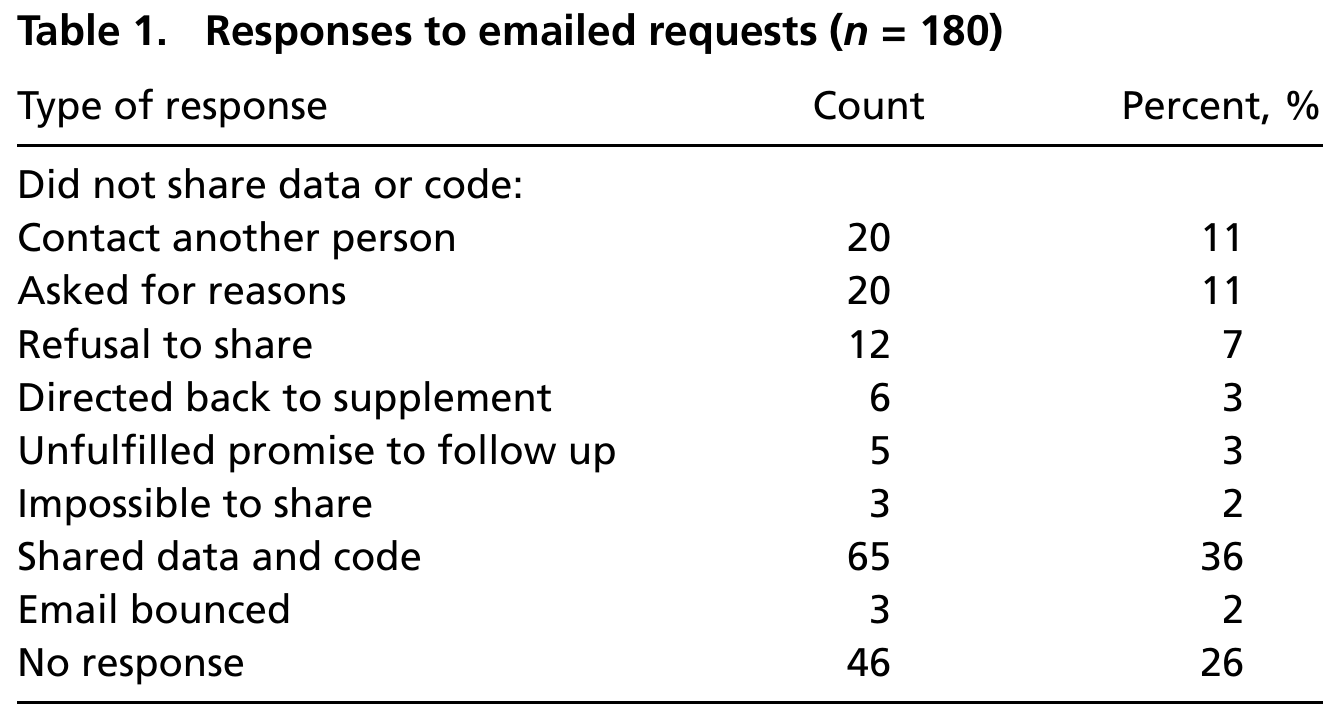
\includegraphics[width=0.9\textwidth]{%
      img/stodden2018_table1.png} %
  \end{figure}

  \vspace{0.1cm}
  
  \begin{center}
    $\Rightarrow$ Code \& data could be retrieved for 91 out of 206 studies.    
  \end{center}

  \source{\cite{Stodden2018}}
  
\end{frame}


\begin{frame}{}%Open Source for Neuroscience}

  \begin{figure}
    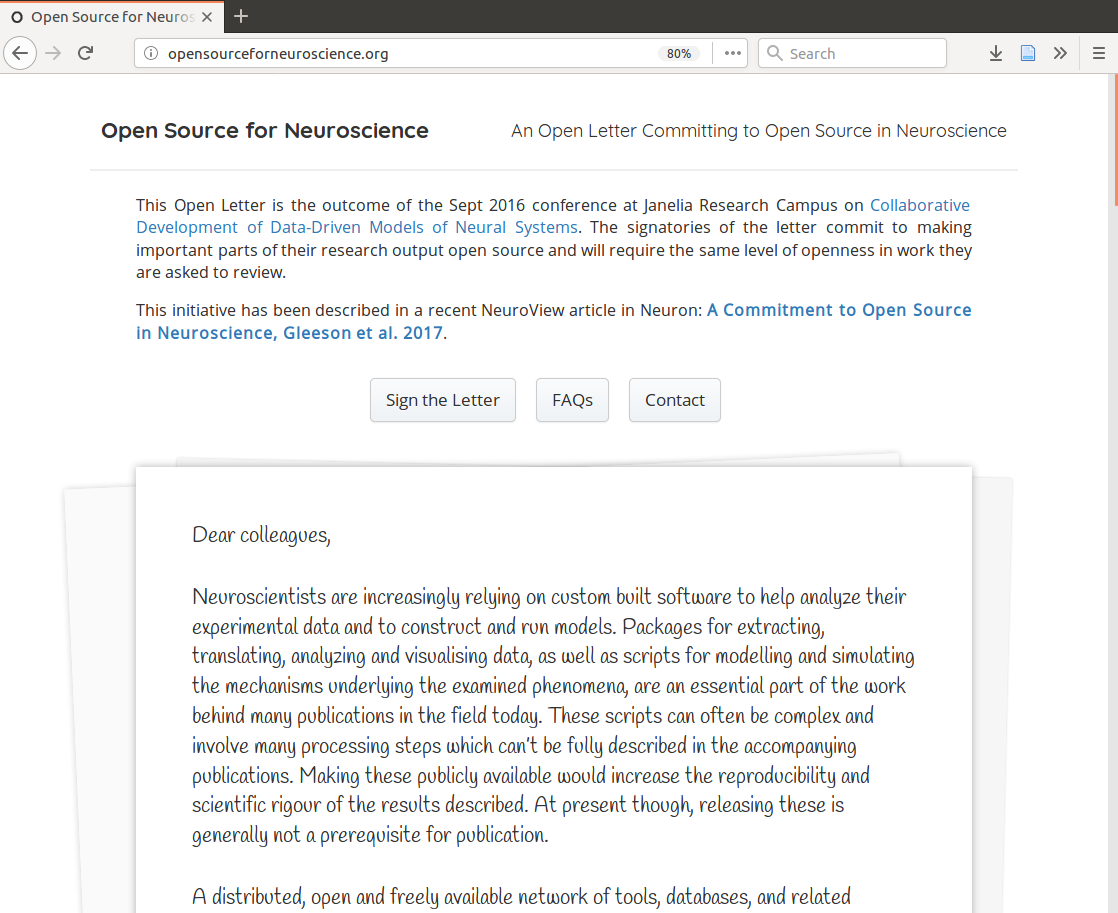
\includegraphics[width=0.95\textwidth]{%
      img/open_source_neuroscience.png} %
  \end{figure}
  
\end{frame}



\begin{frame}{Open Source for Neuroscience}

  \begin{figure}
    \centering
    %% \includegraphics<1>[width=0.9\textwidth]{%
    %%   img/open_source_neuroscience.png} %
    \includegraphics<1>[width=\textwidth]{%
      img/pledge_2.png} %
    \includegraphics<2>[width=\textwidth]{%
      img/pledge_2_t1.png} %
  \end{figure}

  \onslide<1->
  \begin{center}
    \href{http://opensourceforneuroscience.org/}{opensourceforneuroscience.org/}
  \end{center}

  \pnote{
    
    As of 2018/04: 200 neuroscientist have made this pledge
    
  }
  
\end{frame}



\begin{frame}{A slide of hope}

  Researchers are committing to sharing the code and data. Journals have to demand

  This is .

  With this reproducibility in computational research is no longer an issue, right?
  
  
\end{frame}




\begin{frame}{Reproducibility when code was available}

  \vspace{0.05cm}
  
  56 out of 91 studies were judged as \textit{potentially reproducible}

  \vfill
  
  \onslide<2->
  \begin{tabular}{|p{0.9\textwidth}}
    However, even when code was available, more than half of studies were reproducible only with \textit{\textcolor{red}{significant effort!}}  
  \end{tabular}	     

  \vfill


  \onslide<3-6>{

    Problems:
  \vspace{-0.15cm}

  \begin{columns}[T]
    %
    \begin{column}{.5\textwidth}
      %% \minipage[c][0.3\textheight][s]{\columnwidth}
      \begin{itemize}[leftmargin=0.75cm]

      \item<3->[-] impossible to reproduce (missing code, data or methodology)
      \item<4->[-] required tedious effort (e.g.\ download large number of individual data sets)
        
        
      \end{itemize}
      %% \endminipage      

    \end{column}
    %
    \begin{column}{.5\textwidth}
      %% \minipage[c][0.3\textheight][s]{\columnwidth}
      
      \begin{itemize}[leftmargin=*]
      \item<5->[-] required intellectual effort (e.g.\ knowledge of past articles, implementing given pseudo code)
      \item<6->[-] required tweaking (e.g.\ mising parameters, minor methods steps)
            
      \end{itemize}
      %% \endminipage
      
    \end{column}
    %
  \end{columns}
  \vspace{0.2cm}}

  \source{\cite{Stodden2018}}
    
\end{frame}



\begin{frame}{Reproducibility when code was available}

    \begin{figure}
      \centering
      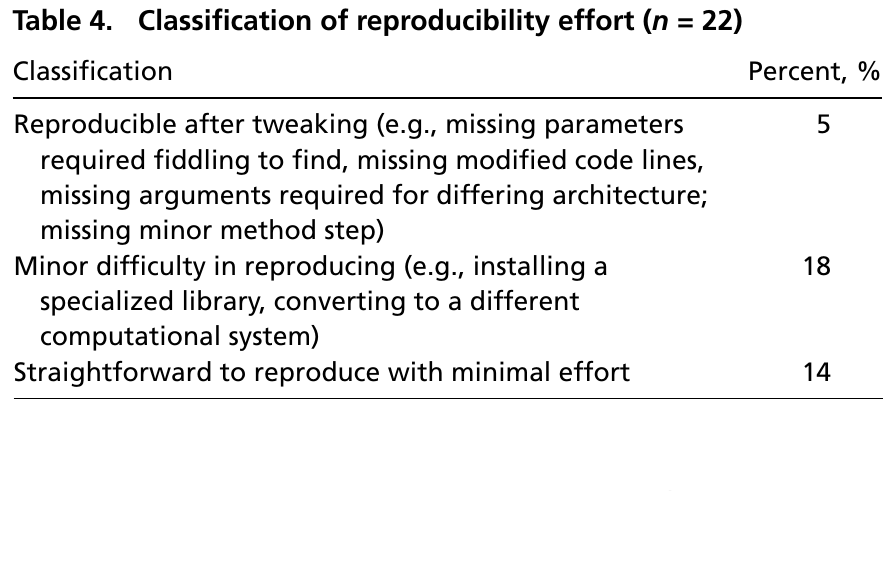
\includegraphics[width=0.85\textwidth]{%
      img/stodden2018_table4_3-3.png} %
    \end{figure}

    \vspace{-1.25cm}
  
\begin{center}
      Computational reproducibility remains difficult even \\when code is available!
      
\end{center}
  
    
\end{frame}






\begin{frame}{\large Measuring Reproducibility in Computer Systems Research}

  \begin{figure}
    \centering
    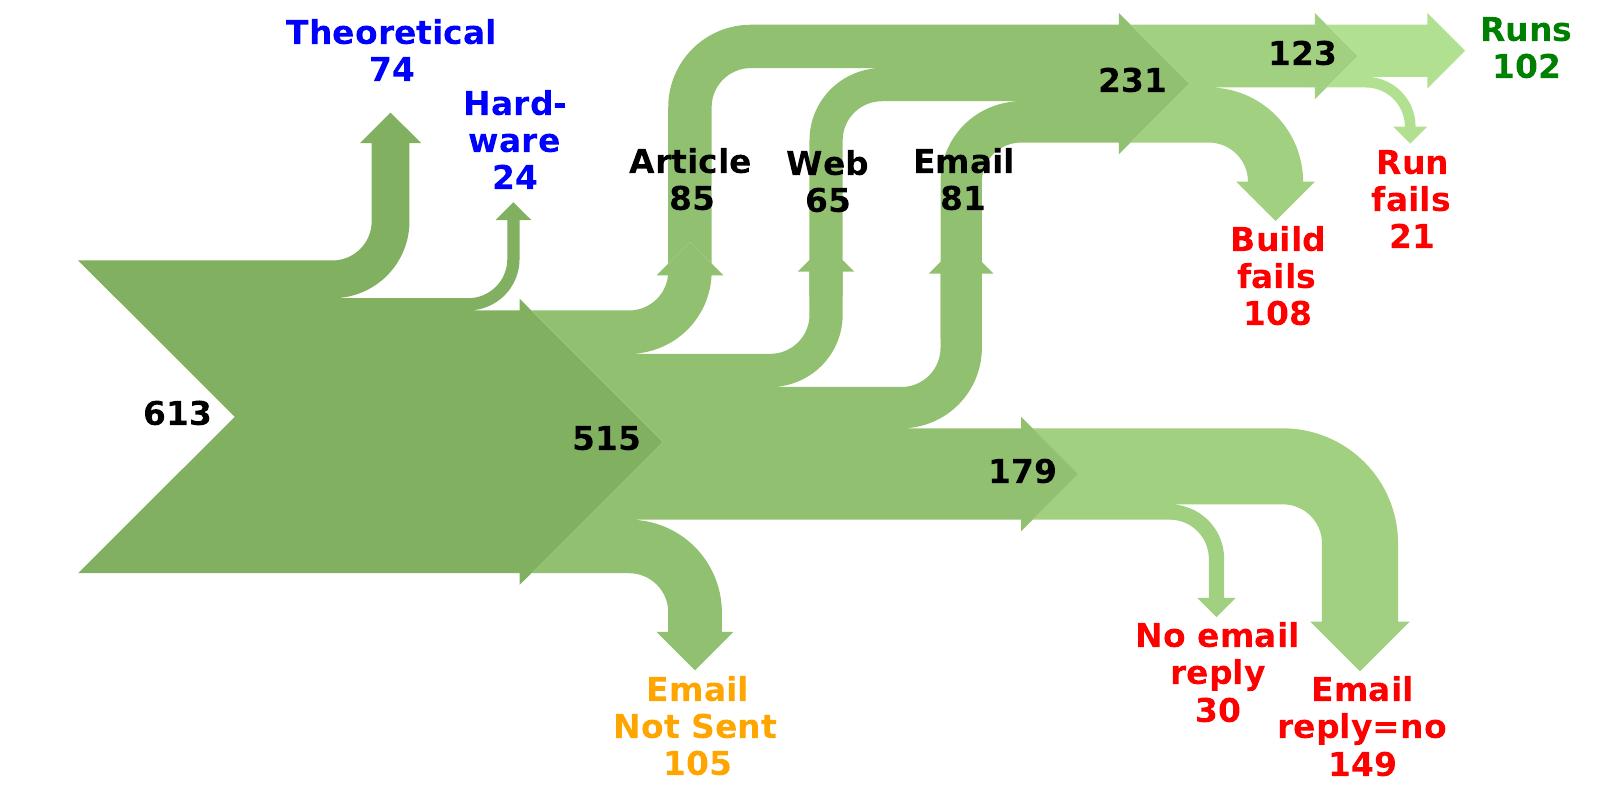
\includegraphics[width=\textwidth]{%
      img/collberg2013_results3.png} %
  \end{figure}
  

  \source{\cite{Collberg2013}}

  \pnote{
    
    613 papers from \\
    - 8 conferences \\
    - 5 journals

    30 minutes of programmer time to try \\
    make build compile/run
    
    Orange: Don't send more than one email to any author \\
    (if author had multiple publications)

    Even if build runs does not even try verify results! \\
    How many more papers will fall off?
    
  }
  
  
\end{frame}


\begin{frame}{}
  
  \begin{figure}
    \centering
    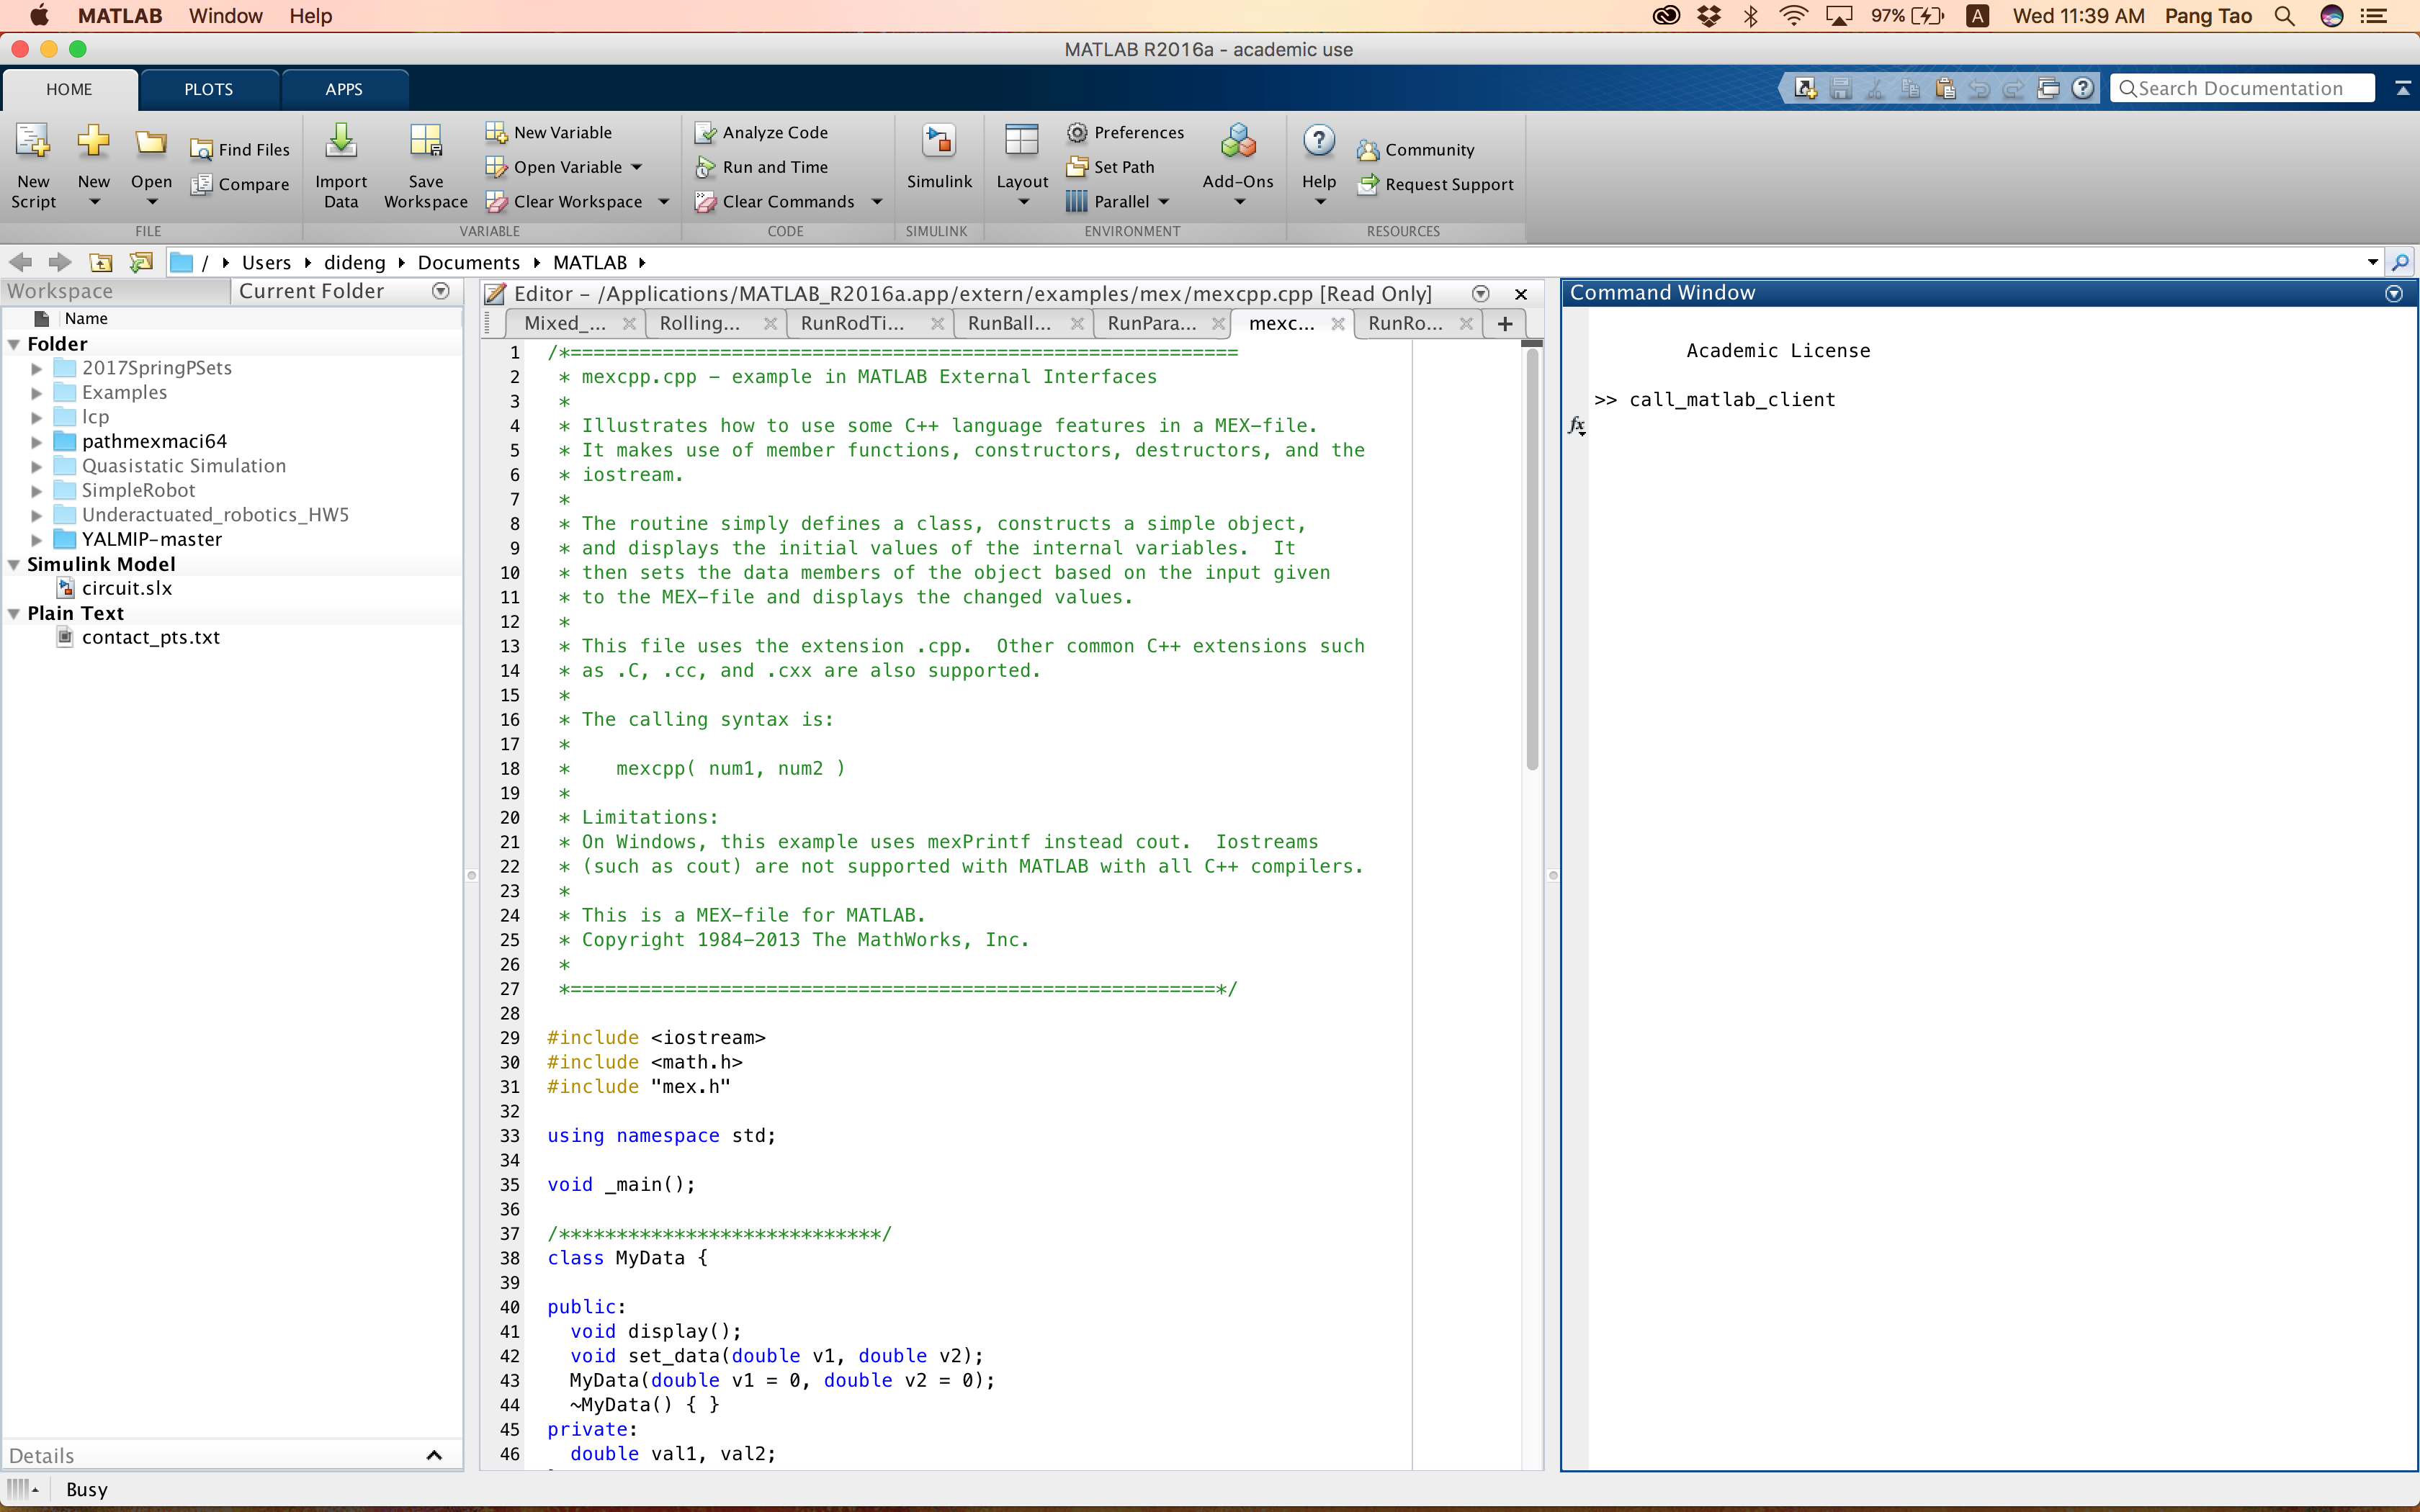
\includegraphics[width=0.95\textwidth]{%
    img/matlab.png} %
  \end{figure}

  \begin{center}
  \large How to publish our research so that (computational) results are reproducible?    
  \end{center}
  
\end{frame}







%% % So what's there to do?
%% % ---> Be open, be reproducible (in that order)
%% % many people are already doing it?
%% % ---> open source for Neuroscience (idea: highlight
%% % researchers from Bordeaux/Frankfurt?)
%% \begin{frame}{Open Source for Neuroscience}

  \begin{figure}
    \centering
    \includegraphics<1>[width=0.9\textwidth]{%
      img/open_source_neuroscience.png} %
    \includegraphics<2>[width=0.9\textwidth]{%
      img/pledge.png} %
    \includegraphics<3>[width=0.9\textwidth]{%
      img/pledge_underline.png} %
  \end{figure}

  \onslide<2->
  \begin{center}
    \href{http://opensourceforneuroscience.org/}{opensourceforneuroscience.org/}
  \end{center}
  

  
  
\end{frame}




%% % Is this at all possible to implement?  Does it
%% % really work? Yes! I think. Here's an example
%% % how things can be done --> My project

%% 
\begin{frame}{A complex computational study - Reproducible?}

  \begin{figure}
    \centering
    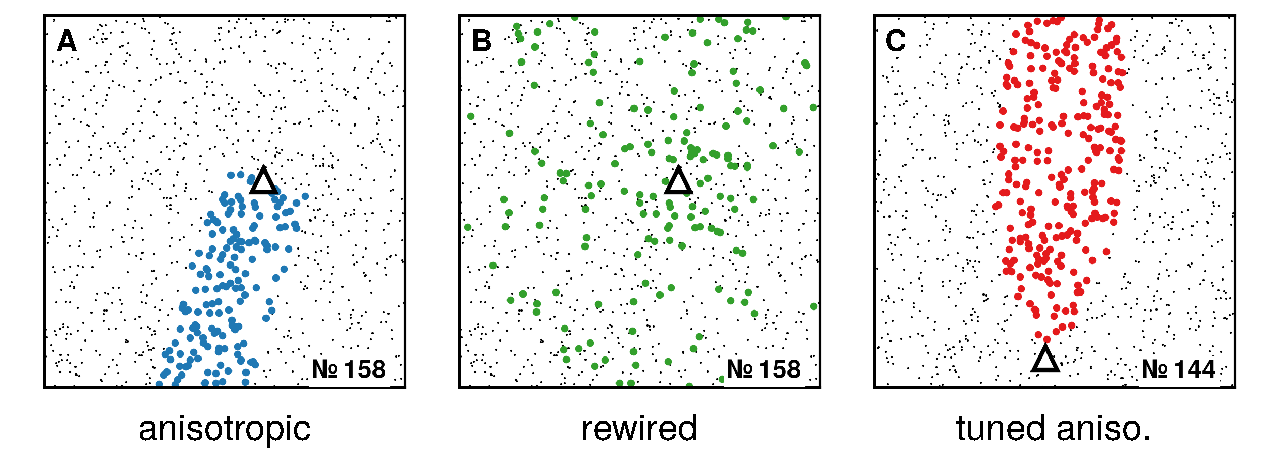
\includegraphics[width=0.85\textwidth]{%
    img/4_network_models_single_row.pdf} %
  \end{figure}

  \vspace{-0.3cm}
  
  \begin{figure}
    \centering
    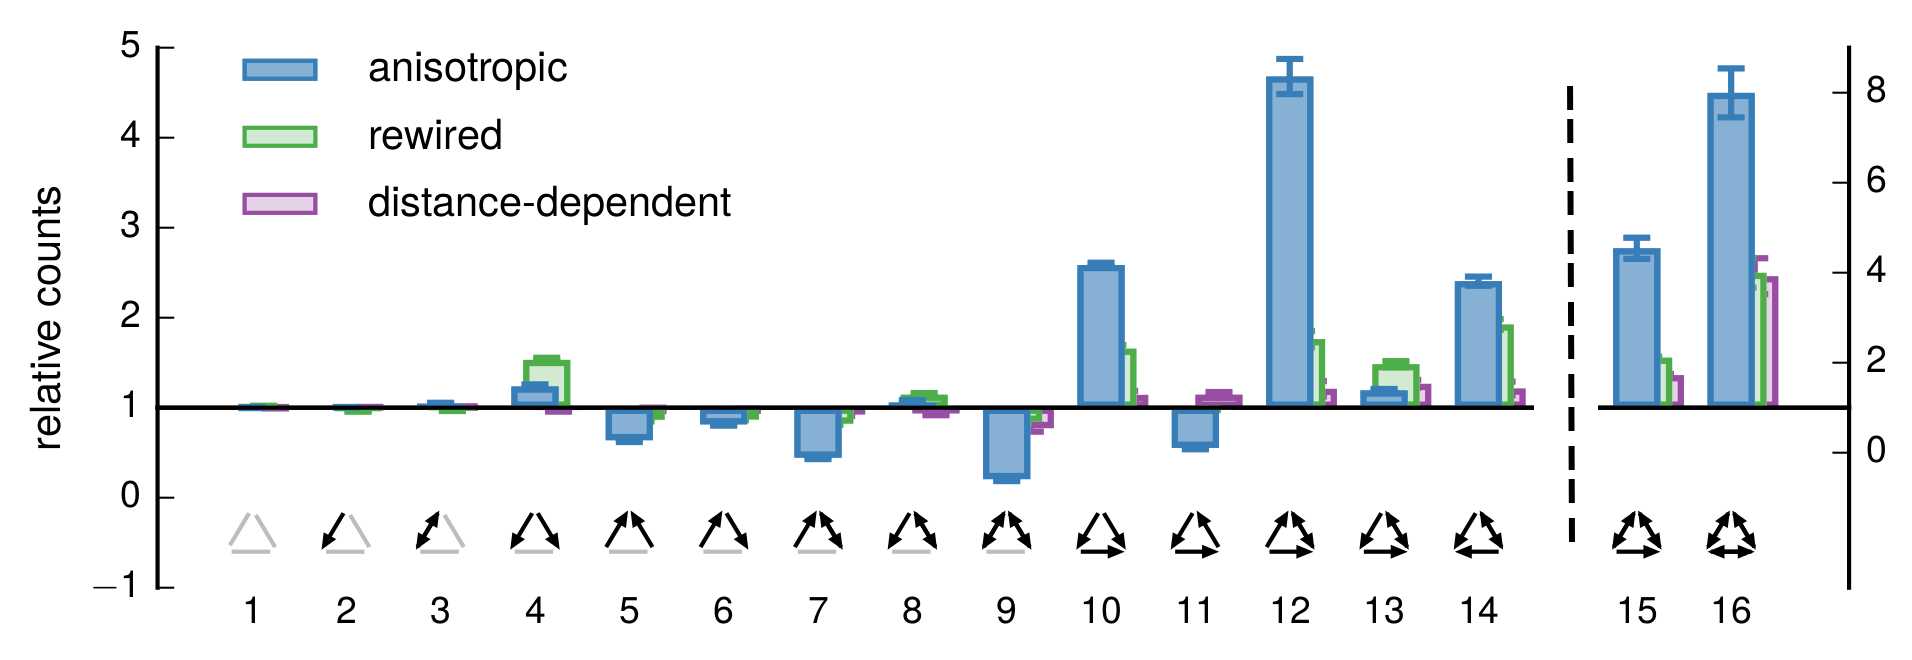
\includegraphics[width=0.9\textwidth]{%
    img/song_motif_single_img_colors.png} %
  \end{figure}

  \pnote{
    
    What makes my study complex:

    - long computations

    - first generation of networks,\\
    then analysis on the generated \\
    networks
    
    
  }
 
  
\end{frame}



%% 

\begin{frame}{Wikimedia Open Science Fellowship}

  %% - picture of the current fellows
  \begin{figure}
    \centering
    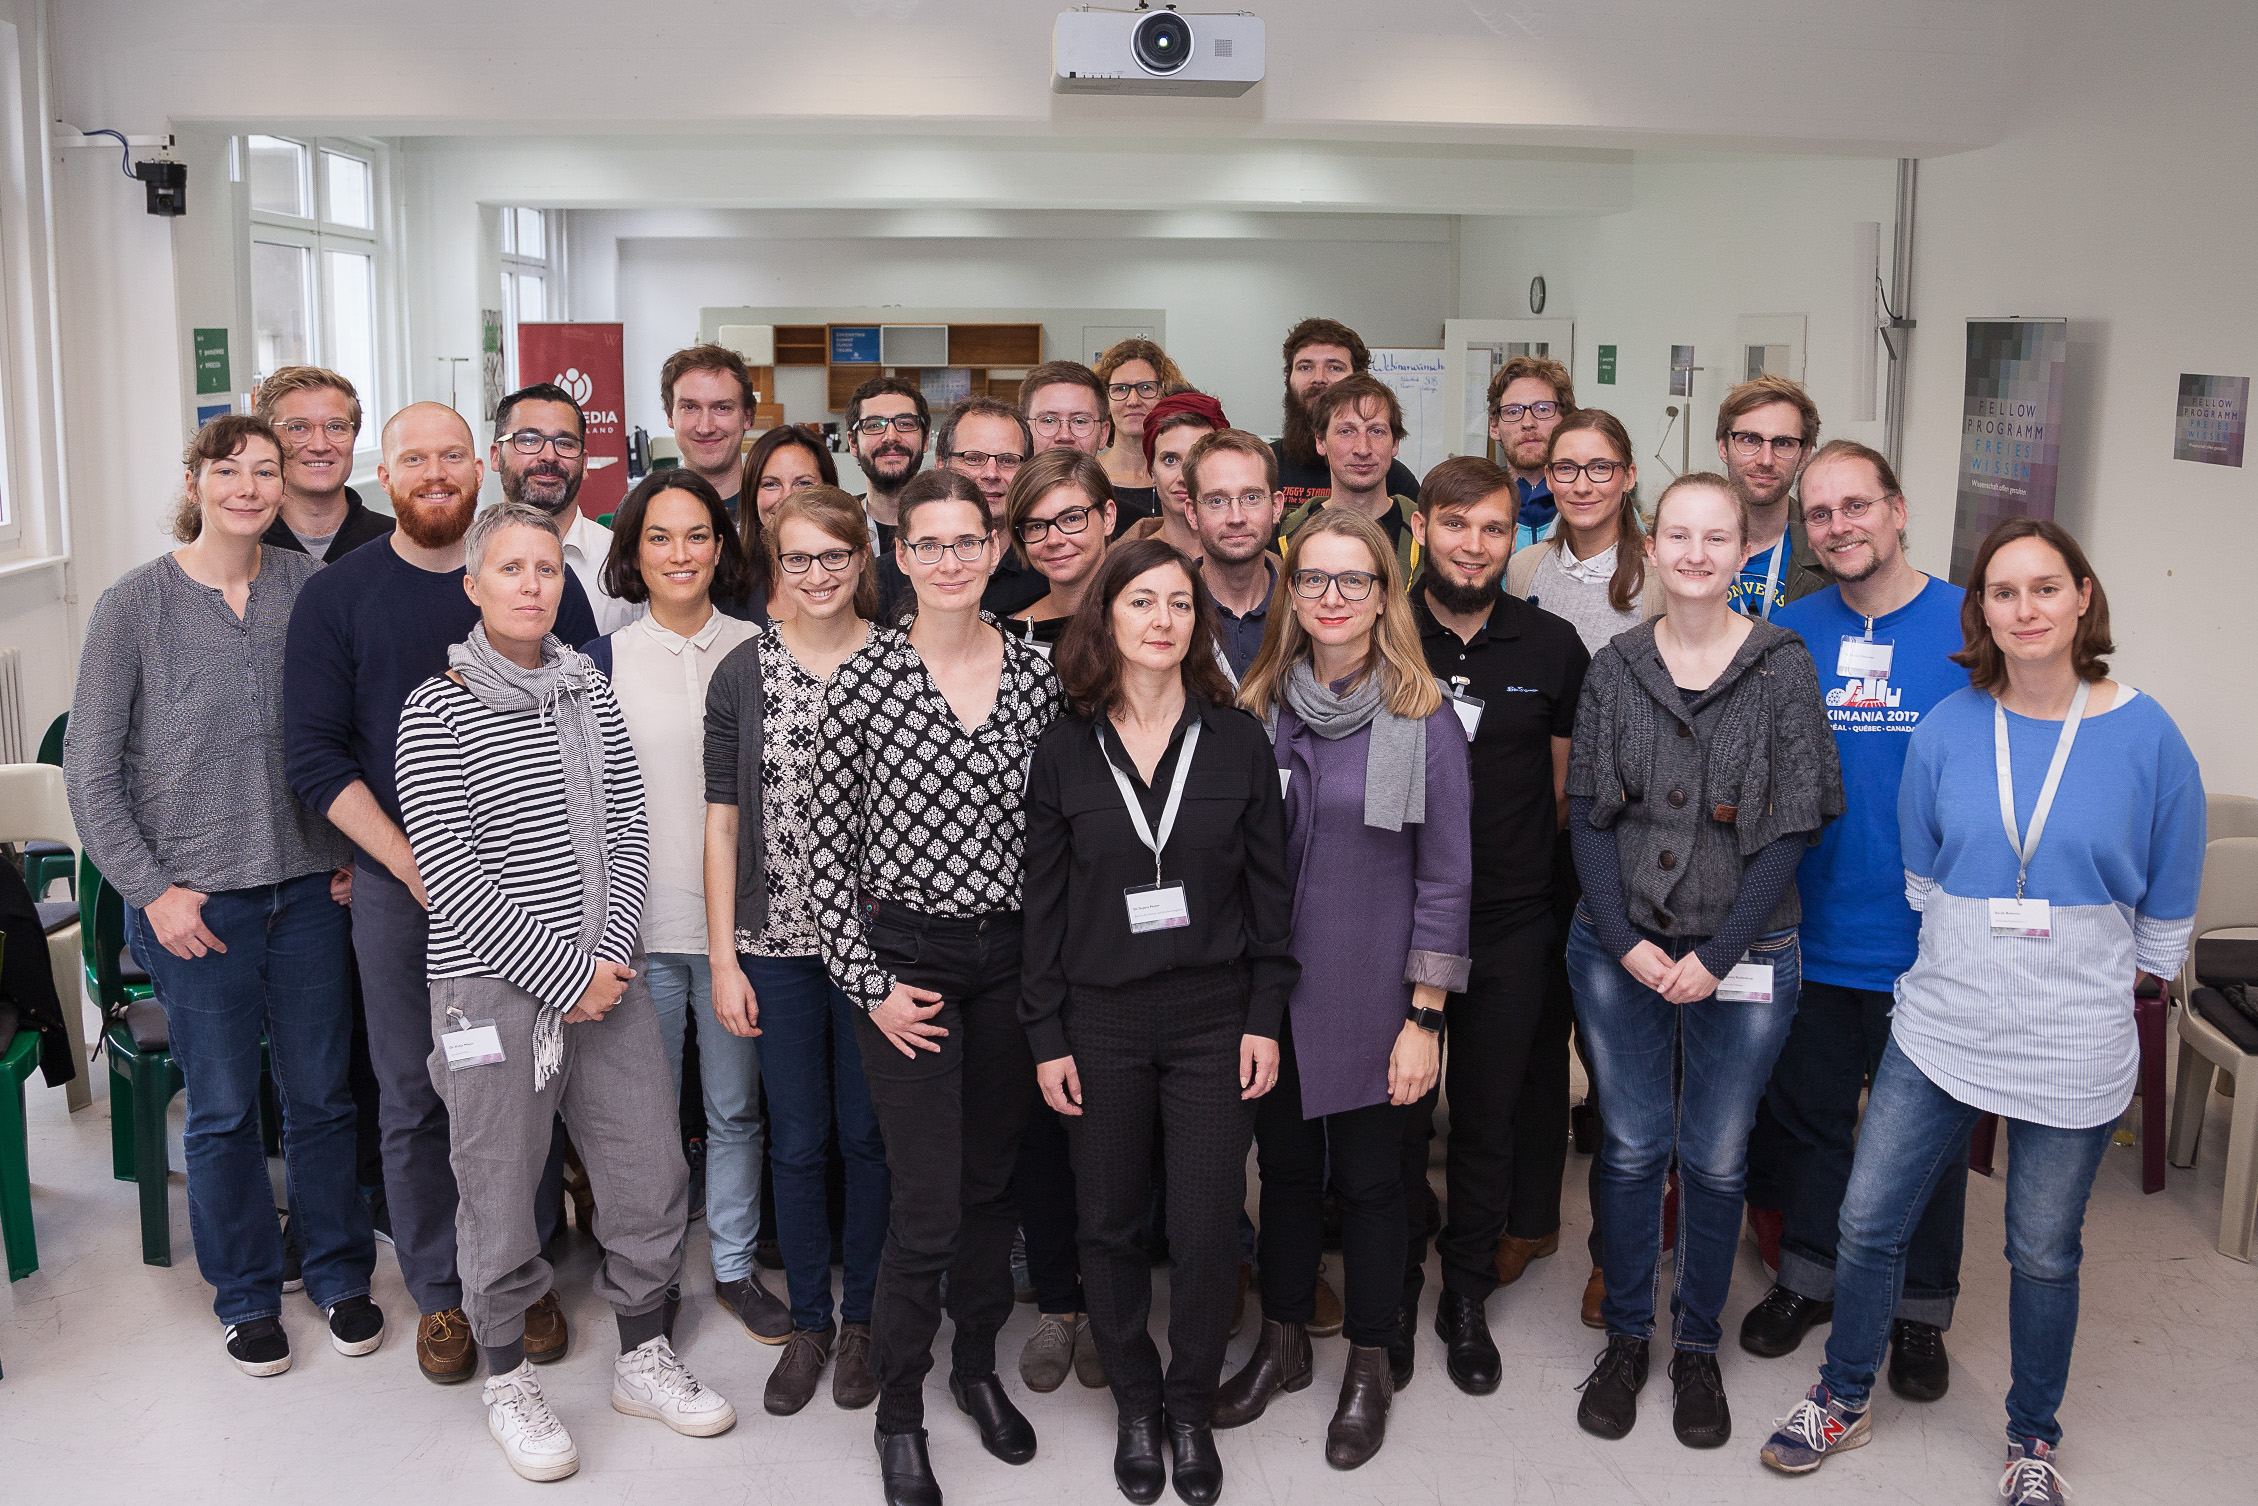
\includegraphics[width=0.875\textwidth]{%
    img/WOSF2017.jpg} %
  \end{figure}
  

  \source{\tiny Photo: Ralf Rebmann, CC BY-SA 4.0}


\end{frame}




\begin{frame}{Wikimedia Open Science Fellowship}

  % 
  \begin{columns}
    %
    \begin{column}{.55\textwidth}


      \begin{figure}
        \centering
        
\includegraphics[width=0.96\textwidth]{%
        img/logo_wosf_full.png} %
      \end{figure}
      

      
      

    \end{column}
    %
    \begin{column}{.45\textwidth}
      \minipage[c][0.625\textheight][s]{\columnwidth}

      \vspace{0.2cm}
      
      \begin{itemize}[leftmargin=*]

      \item[-] runs from October to June

      \item[-] fellows are paired with a mentor who supports the progress

      \item[-] financial support offered

      \item[-] program in German

      \item[-]       application for 3rd round now open!
      \href{http://bit.ly/osfprog}{bit.ly/osfprog}


      \end{itemize}

      

      \endminipage      
    \end{column}
  \end{columns}
  
\end{frame}





%% \begin{frame}{Problems to solve}
  %

  \vspace{-0.5cm}
  
  \begin{columns}
    %
    \begin{column}{.6\textwidth}
      \minipage[c][0.2\textheight][s]{\columnwidth}

      \vfill
      
      Problem 1 \onslide<2->{Check}

      \begin{itemize}[leftmargin=0.6cm]
        
      \item[-] using of difficult to install computational environment (graph-tool)       
        
      \end{itemize}

      \vfill
      
      
      \endminipage      
    \end{column}
    %
    \begin{column}{.4\textwidth}



      \begin{figure}
        \centering
        
\includegraphics[width=0.75\textwidth]{%
          img/docker_logo.pdf} %
      \end{figure}
      



      
    \end{column}
  \end{columns}


  \onslide<3->
  \vspace{-0.3cm}
  \begin{columns}
    %
    \begin{column}{.6\textwidth}
      \minipage[c][0.5\textheight][s]{\columnwidth}

      \vfill
      
      Problem 2        

      \begin{itemize}[leftmargin=0.6cm]
        
      \item<3->[-] long \& resource demanding computations
      \item<4->[-] subsequent analysis require output of previous computations \vspace{0.17cm}
      \item<5->[] \textit{difficult to understand what is required to reproduce a single output (1 figure)}
        
      \end{itemize}


      
      \endminipage      
    \end{column}
    %
    \begin{column}{.4\textwidth}
      \vspace{0.1cm}
      \begin{figure}
        \centering
        \includegraphics<6->[width=0.85\textwidth]{%
          img/sumatra_logo.png} %
      \end{figure}

      
      
      
    \end{column}
  \end{columns}  
\end{frame}



%% \include{frames/docker}

%% \include{frames/Sumatra}

%% \begin{frame}{}
%%   \begin{center}
%%     \begin{tikzpicture}[remember picture,overlay]
%%       \node[anchor=center, inner sep=0pt] at (current page.center) {%
%%         \movie[autostart,width=0.85\paperwidth, height = 0.6852577319587629\paperwidth, poster] {}{gif/docker.mp4}%
%%       };
%%     \end{tikzpicture}
    
%%   \end{center}
%% \end{frame}


\begin{frame}{}
  
  \begin{center}
    \inlineMovie[autostart&start=0.&stop=5.9]{movie/docker.mp4}{movie/docker01.png}{height=0.9\textheight}

  \end{center}
  
\end{frame}


\begin{frame}{}
  
  \begin{center}
    \inlineMovie[autostart&start=6.4&stop=18.5]{movie/docker.mp4}{movie/docker02.png}{height=0.9\textheight}

  \end{center}
  
\end{frame}



\begin{frame}{}
  
  \begin{center}
    \inlineMovie[autostart&start=19.9]{movie/docker.mp4}{movie/docker03.png}{height=0.9\textheight}

  \end{center}
  
\end{frame}



\begin{frame}{}
  
  \begin{center}
    \inlineMovie[autostart]{movie/smtweb.mp4}{movie/smtweb.png}{height=0.9\textheight}

  \end{center}
  
\end{frame}



\begin{frame}{}
  
  \begin{center}
    \inlineMovie[autostart]{movie/smt_repeat.mp4}{movie/smt_repeat.png}{height=0.9\textheight}

  \end{center}
  
\end{frame}









%% % A few tips in practice:

%% % -- [1] upload to Zenodo, OSF.io, ---> DOI
%% % -- [2] use random seeds and makefile to regenerate results
%% % -- [3] document versions of code (toolboxes), (pip freeze, MATLAB versions)
%% % -- [4] provide dependencies (Docker, Singularity, Virtual Machine,...)
%% % -- [5] document more closely parameters, input/output, ...
%% \include{frames/in_practice}



%% % So what can I take out of this talk? Give some rules
%% % and guide lines to follow (other resources)?
%% 
\begin{frame}{}

  - Zenodo
  - Open Science Framework
  -  
  
\end{frame}


%% % Next, we need reproducibility! What is even
%% % reproducible? Does open==reproducible?
%% % So what does code need to look like in practice?
%% % --> Rougier's five Rs
%% \begin{frame}{\large Measuring Reproducibility in Computer Systems Research}

  \begin{figure}
    \centering
    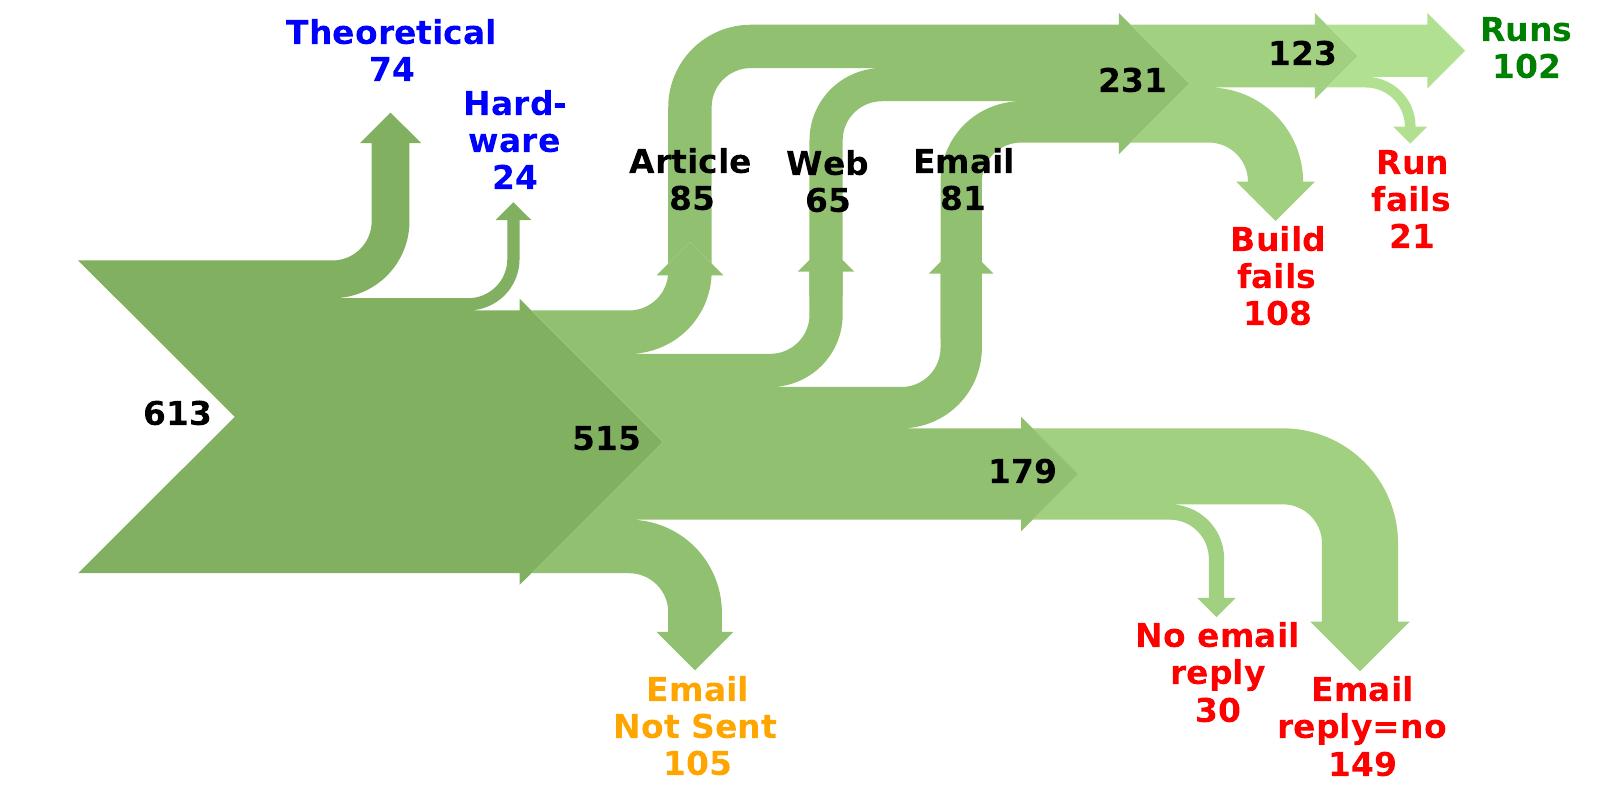
\includegraphics[width=\textwidth]{%
    img/collberg2013_results3.png} %
  \end{figure}
  

  \source{\cite{Collberg2013}}

  \pnote{
    
    613 papers from \\
    - 8 conferences \\
    - 5 journals

    30 minutes of programmer time to try \\
    make build compile/run
    
    Orange: Don't send more than one email to any author \\
    (if author had multiple publications)

    Even if build runs does not even try verify results! \\
    How many more papers will fall off?
    
  }
  
  
\end{frame}

\begin{frame}{}

  \vspace{-0.5cm}
  
  \begin{figure}
    \centering
    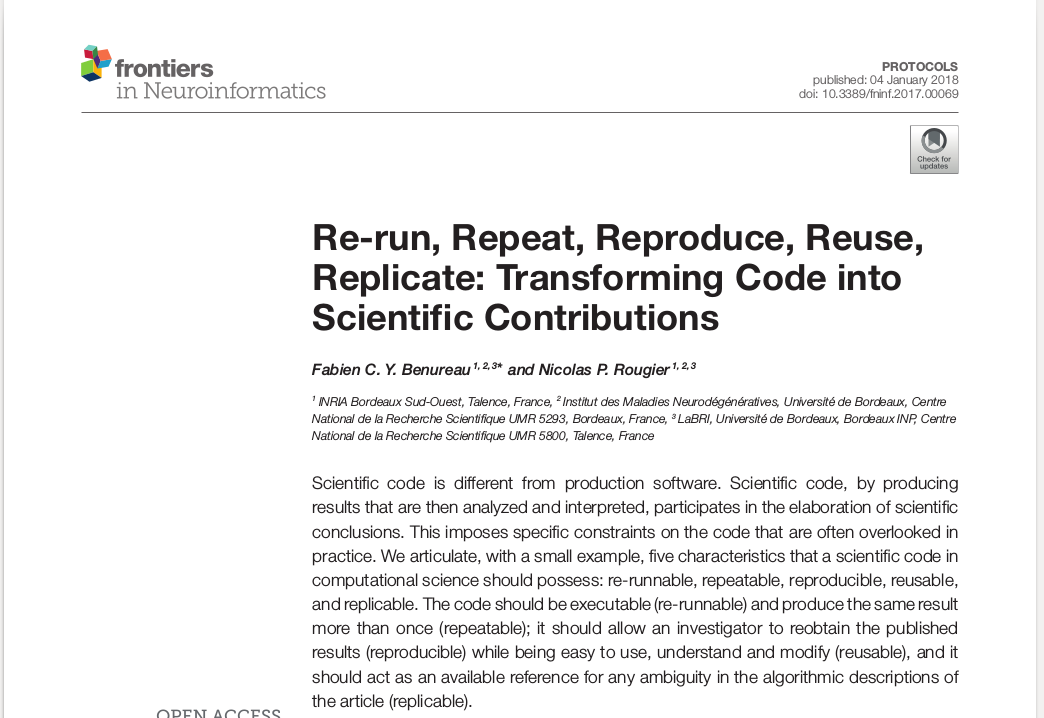
\includegraphics[height=0.785\textheight]{%
    img/benureau2018_cover2.png} %
  \end{figure}
  

  \source{\cite{Benureau2018}}  
  
  
\end{frame}





\begin{frame}{Five \textit{Rs} for scientific code}

  
  \begin{itemize}[leftmargin=2.6cm]
    \itemsep11pt
    \item[$\mathbf{R^1}$ \textit{Re-runnable}:] can be run again when needed (e.g.~more than the one time that was needed to produce the results)

    \item[$\mathbf{R^2}$ \textit{Repeatable}:] program is deterministic, produces repeatable output

    \item[$\mathbf{R^3}$ \textit{Reproducible}:] another researcher can take code \& input data, execute code, and re-obtain same results

    \item[$\mathbf{R^4}$ \textit{Reusable}:] program  can be easily used, and
modified, by you and other people, inside \& outside own lab

    \item[$\mathbf{R^5}$ \textit{Replicable}:] program can be re-implemented by another research to re-obtain results

  \end{itemize}

  

  
  \source{\cite{Benureau2018}}
  
  
\end{frame}



\begin{frame}{$R^0$ -- runnable code}

  \begin{figure}
    \centering
    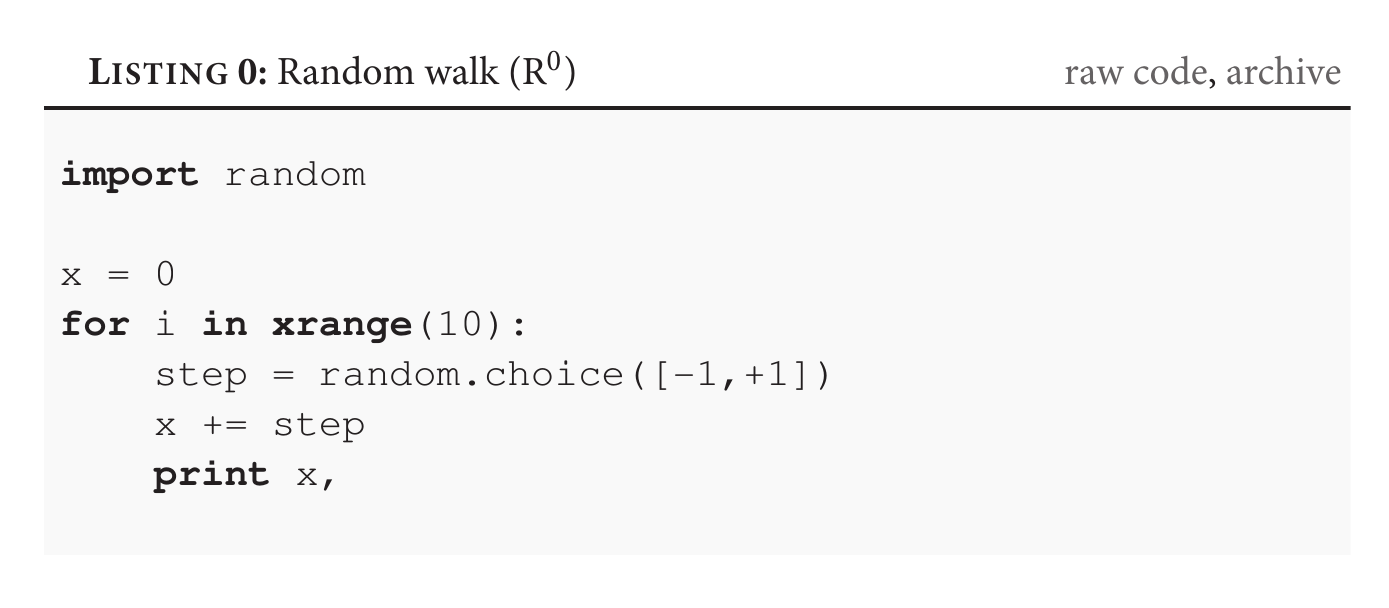
\includegraphics[width=\textwidth]{%
      img/R0_code.png} %
  \end{figure}

  \begin{figure}
    \centering
    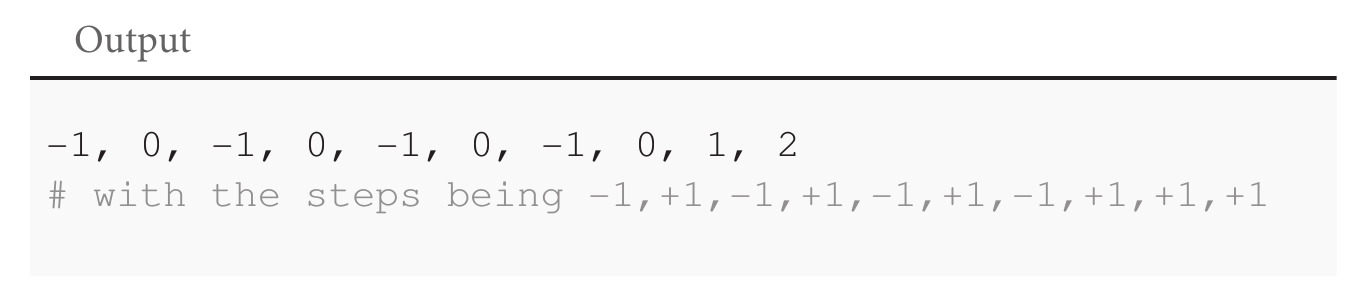
\includegraphics[width=\textwidth]{%
      img/R0_output.png} %
  \end{figure}

  \vspace{1.5cm}  

  \source{\cite{Benureau2018}}
  
  
\end{frame}



\begin{frame}{$R^1$ -- Re-runnable}

  \begin{figure}
    \centering
    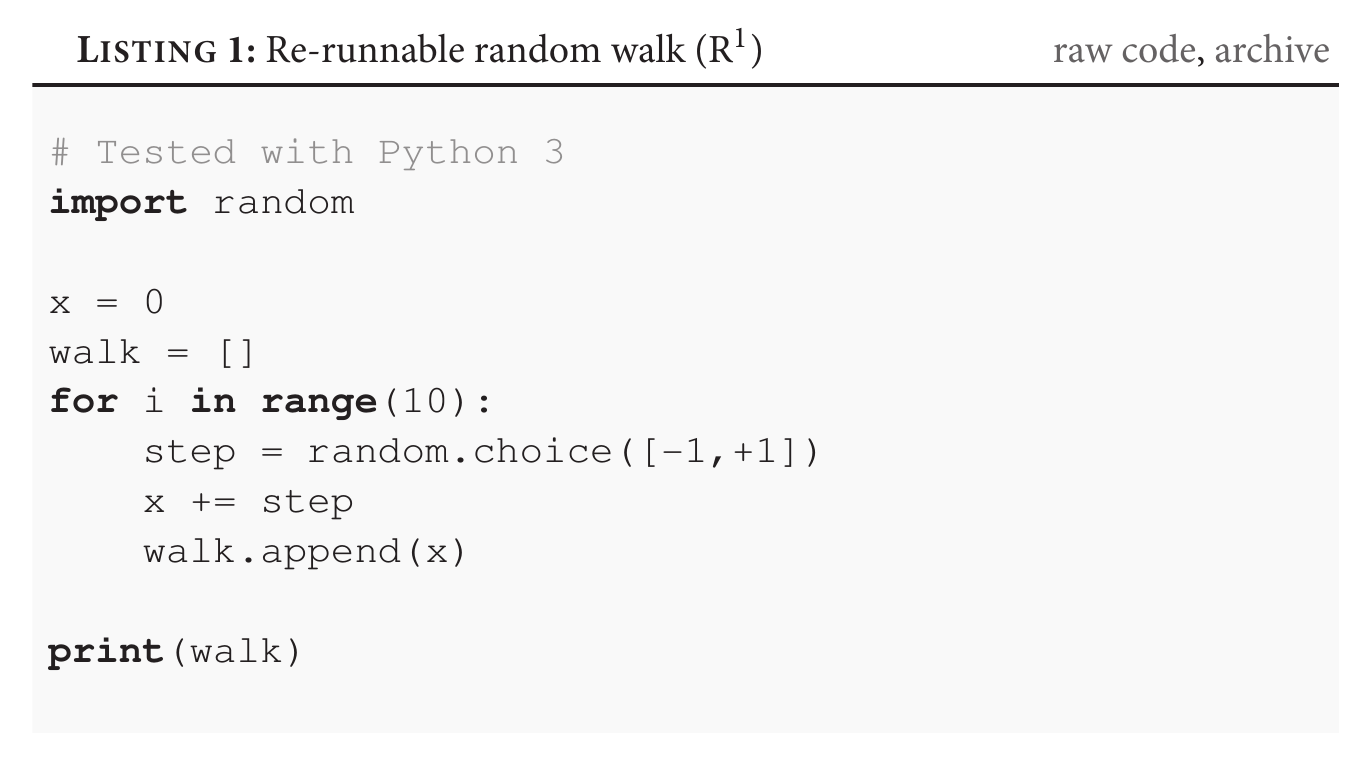
\includegraphics[width=\textwidth]{%
      img/R1_code.png} %
  \end{figure} 
  
  
\end{frame}

\begin{frame}{$R^2$ -- Repeatable}
  
  
  
\end{frame}



\begin{frame}{$R^3$ -- Reproducible}

  \begin{figure}
    \centering
    \includegraphics<1>[width=.8\textwidth]{%
      img/R3_code01.png} %
    \includegraphics<2>[width=.8\textwidth]{%
      img/R3_code02.png} %   
  \end{figure}

  \source{\only<1>{1}\only<2>{2}/2}
    
\end{frame}


\begin{frame}{$R^4$ -- Reusable}

  \begin{figure}
    \centering
    \includegraphics<1>[width=.8\textwidth]{%
      img/R4_code01.png} %
    \includegraphics<2>[width=.8\textwidth]{%
      img/R4_code02.png} %
    \includegraphics<3>[width=.8\textwidth]{%
      img/R4_code03.png} %   
  \end{figure}

    \source{\only<1>{1}\only<2>{2}\only<3>{3}/3}
    
\end{frame}


\begin{frame}{$R^5$ -- Replicable}

  \begin{figure}
    \centering
    \includegraphics<1>[width=.8\textwidth]{%
      img/R5_code01.png} %
    \includegraphics<2>[width=.8\textwidth]{%
      img/R5_code02.png} %   
  \end{figure}

  \source{\only<1>{1}\only<2>{2}/2}
    
\end{frame}



%% \begin{frame}[t]{References \hspace{3.25cm} }

  \begin{multicols}{2}
    \printbibliography
  \end{multicols}
  \vspace{0.25cm}
  \begin{center}
    \LARGE
    \textit{Thank you!}
  \end{center}

  \pnote {

  }
  
\end{frame}


%% 

\begin{frame}{$R^0$ -- runnable code}

  \begin{figure}
    \centering
    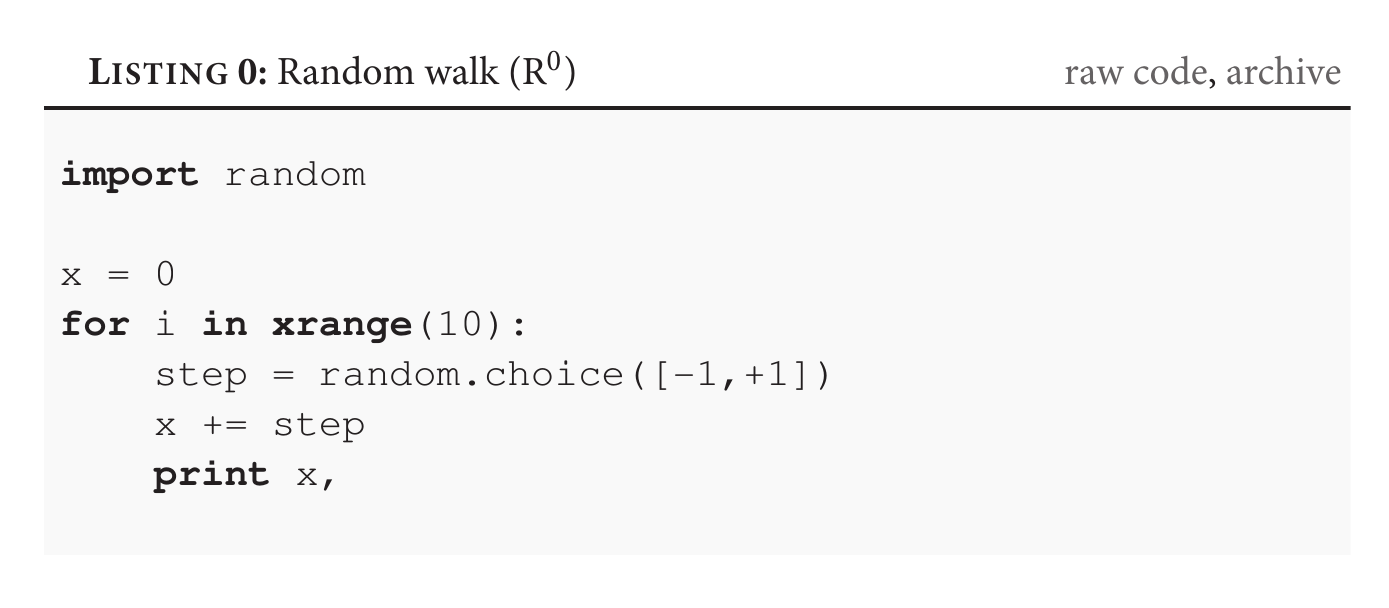
\includegraphics[width=\textwidth]{%
      img/R0_code.png} %
  \end{figure}

  \begin{figure}
    \centering
    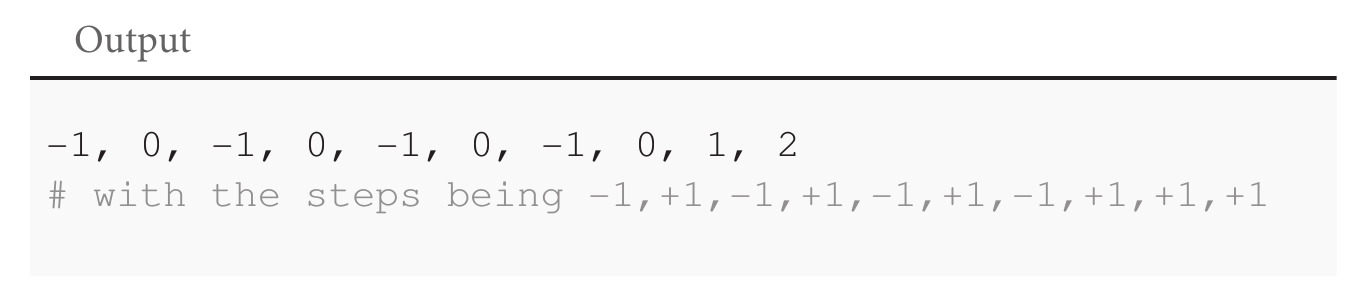
\includegraphics[width=\textwidth]{%
      img/R0_output.png} %
  \end{figure}

  \vspace{1.5cm}  

  \source{\cite{Benureau2018}}
  
  
\end{frame}



\begin{frame}{$R^1$ -- Re-runnable}

  \begin{figure}
    \centering
    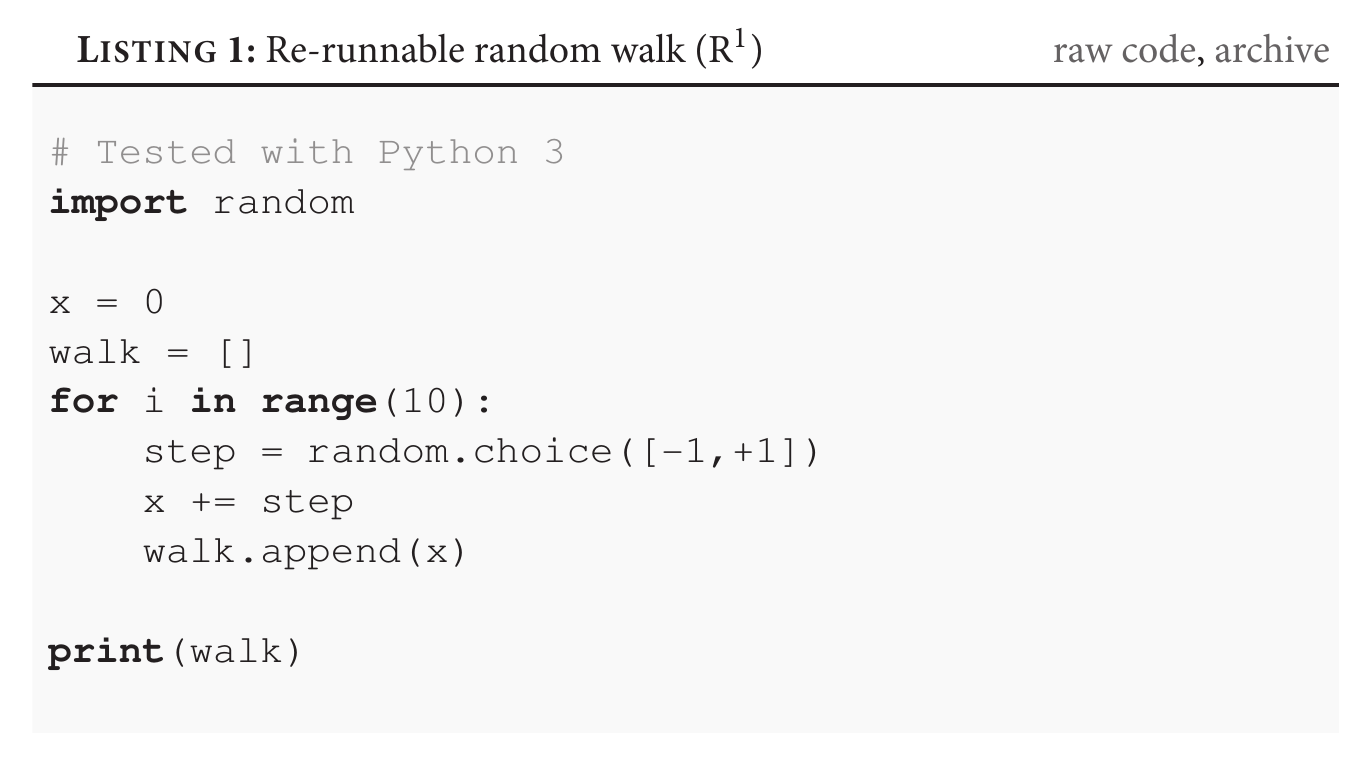
\includegraphics[width=\textwidth]{%
      img/R1_code.png} %
  \end{figure} 
  
  
\end{frame}



\begin{frame}{$R^2$ -- Repeatable}
  
    \begin{figure}
    \centering
    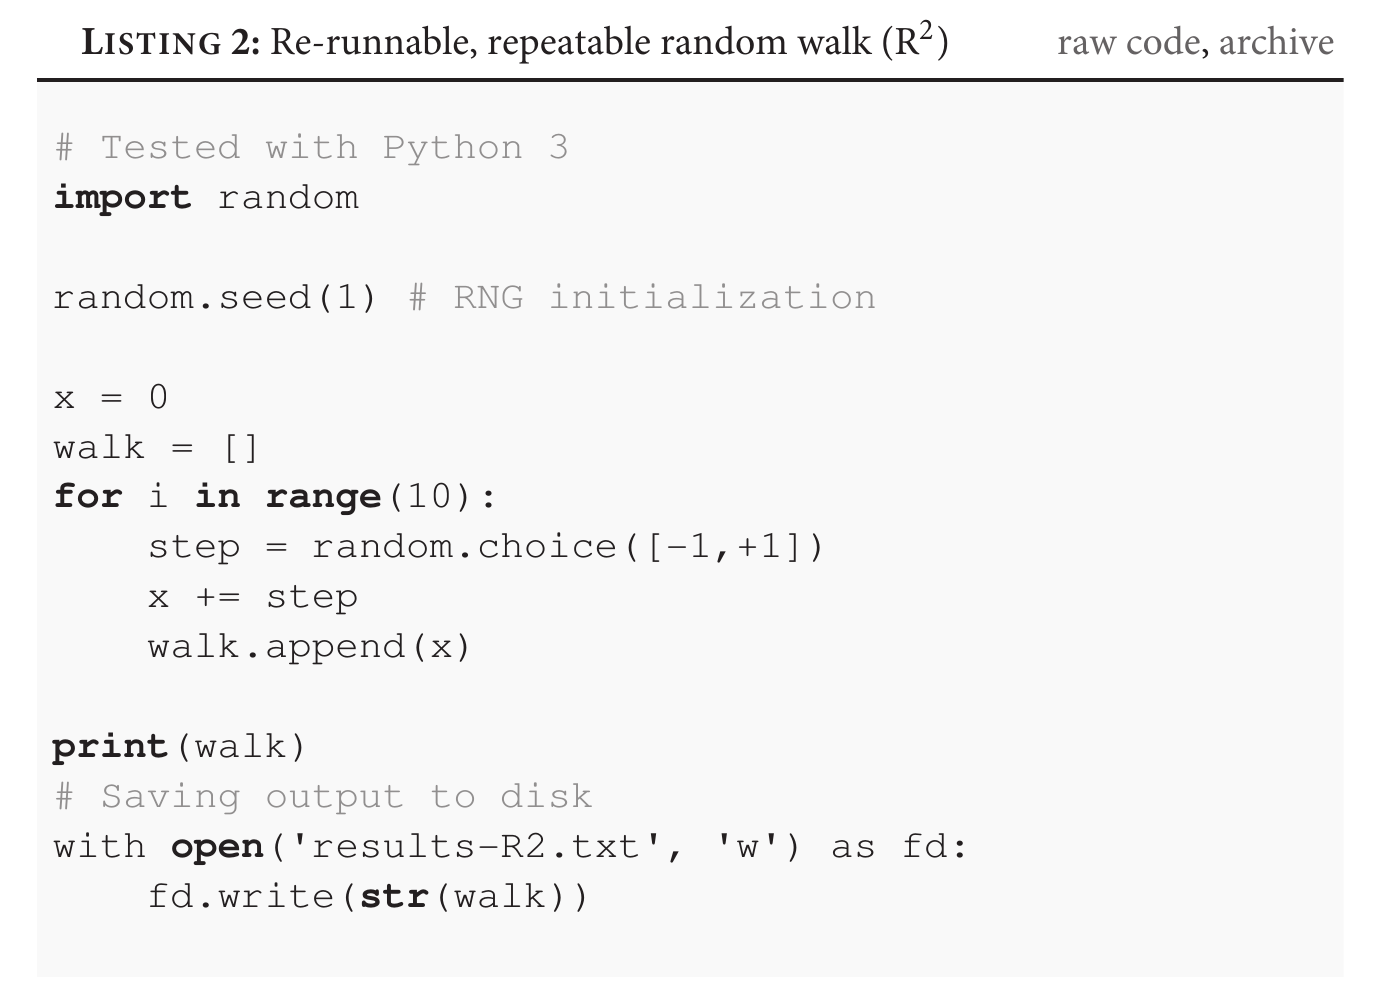
\includegraphics[width=\textwidth]{%
      img/R2_code.png} %
    \end{figure} 
      
\end{frame}



\begin{frame}{$R^3$ -- Reproducible}

  \begin{figure}
    \centering
    \includegraphics<1>[width=.8\textwidth]{%
      img/R3_code01.png} %
    \includegraphics<2>[width=.8\textwidth]{%
      img/R3_code02.png} %   
  \end{figure}

  \source{\only<1>{1}\only<2>{2}/2}
    
\end{frame}


\begin{frame}{$R^4$ -- Reusable}

  \begin{figure}
    \centering
    \includegraphics<1>[width=.8\textwidth]{%
      img/R4_code01.png} %
    \includegraphics<2>[width=.8\textwidth]{%
      img/R4_code02.png} %
    \includegraphics<3>[width=.8\textwidth]{%
      img/R4_code03.png} %   
  \end{figure}

    \source{\only<1>{1}\only<2>{2}\only<3>{3}/3}
    
\end{frame}



\begin{frame}{$R^5$ -- Replicable}

  \begin{figure}
    \centering
    \includegraphics<1>[width=.8\textwidth]{%
      img/R5_code01.png} %
    \includegraphics<2>[width=.8\textwidth]{%
      img/R5_code02.png} %   
  \end{figure}

  \source{\only<1>{1}\only<2>{2}/2}
    
\end{frame}





\end{document}
















